\documentclass[10pt,a4paper,oneside,fleqn]{report}
\usepackage{geometry}
\geometry{a4paper,left=20mm,right=20mm,top=1cm,bottom=2cm}
\usepackage[utf8]{inputenc}
%\usepackage{ngerman}
\usepackage{amsmath}                % brauche ich um dir Formel zu umrahmen.
\usepackage{amsfonts}                % brauche ich für die Mengensymbole
\usepackage{graphicx}
\setlength{\parindent}{0px}
\setlength{\mathindent}{10mm}
\usepackage{bbold}                    %brauche ich für die doppel Zahlen Darstellung (Einheitsmatrix z.B)
\usepackage[linktocpage={false}]{hyperref}


\usepackage{color}
\usepackage{titlesec} %sudo apt-get install texlive-latex-extra

\definecolor{darkblue}{rgb}{0.1,0.1,0.55}
\definecolor{darkred}{rgb}{0.55,0.2,0.2}

\titleformat{\chapter}[display]{\color{darkred}\normalfont\huge\bfseries}{\chaptertitlename\
\thechapter}{20pt}{\Huge}

\titleformat{\section}{\color{darkblue}\normalfont\Large\bfseries}{\thesection}{1em}{}
\titleformat{\subsection}{\color{darkblue}\normalfont\Large\bfseries}{\thesection}{1em}{}

% Notiz Box
\usepackage{fancybox}
\newcommand{\notiz}[1]{\vspace{5mm}\ovalbox{\begin{minipage}{1\textwidth}#1\end{minipage}}\vspace{5mm}}

\usepackage{cancel}


%\includegraphics[width=0.75\textwidth]{thepic.png}

\begin{document}
\tableofcontents
\setcounter{chapter}{12}
\chapter{Supraleitung}

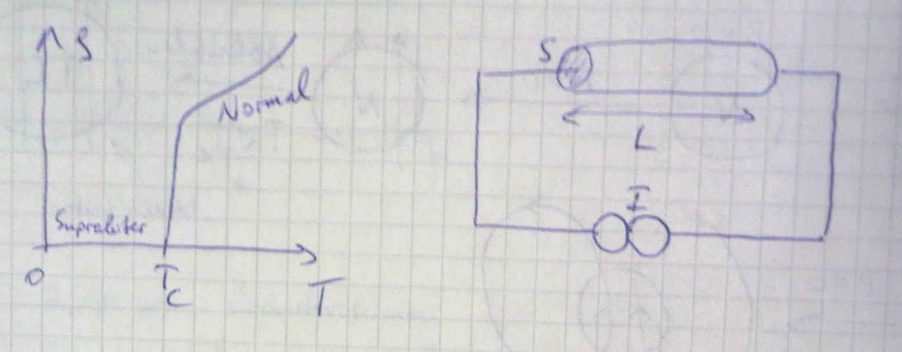
\includegraphics[width=0.75\textwidth]{kap13_01.png}

\[U=RI = \rho\frac{L}{S}I\]

\[\left.\rho\right|_{Cu,T=4,2K}\approx 10^{-9}\Omega m\]

für \(\rho < 10^{-24}\Omega cm\)

1911 Kamerlingli-Onnes

Hg: \(T_c\approx 4K\)

\begin{tabular}{ccc}
  \(N_z\)&\(\rightarrow \)&77K\\
  \(H_z\)&\(\rightarrow \)&20K\\
  \(^4He\)&\(\rightarrow \)&4,2K\\
\end{tabular}

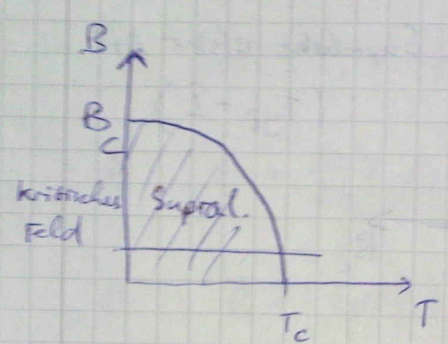
\includegraphics[width=0.45\textwidth]{kap13_02.png}

\begin{tabular}{cc}
  Al&1,2K\\
Im&3,4K\\
Sn&3,7K\\
Pb&7,2K\\
Nb&9,2K\\
--&--\\
NbN&15K\\
\(Nb_3Ge\)&24K\\
1986 \(YBaCu_3O_7\) & 92
\end{tabular}

\(Tl_2Sr_2Ca_2Cu_3O_8 \rightarrow 120K\)

Supralaeiter ist kein 'idealer' Leiter \(\rightarrow \) Meissner-Effekt



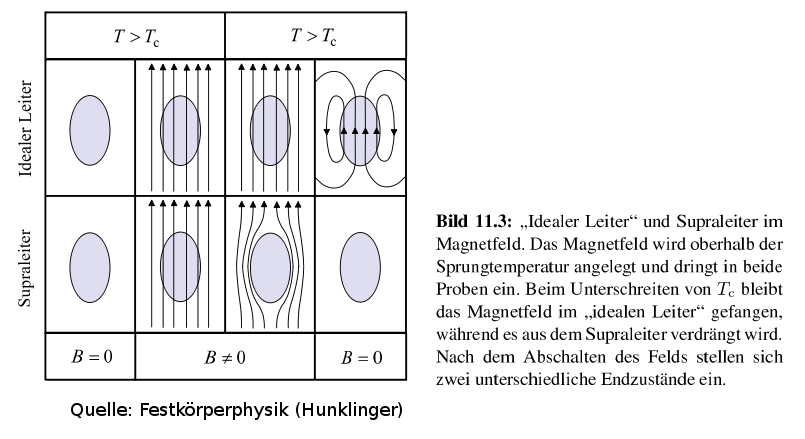
\includegraphics[width=0.75\textwidth]{kap13_03.png}




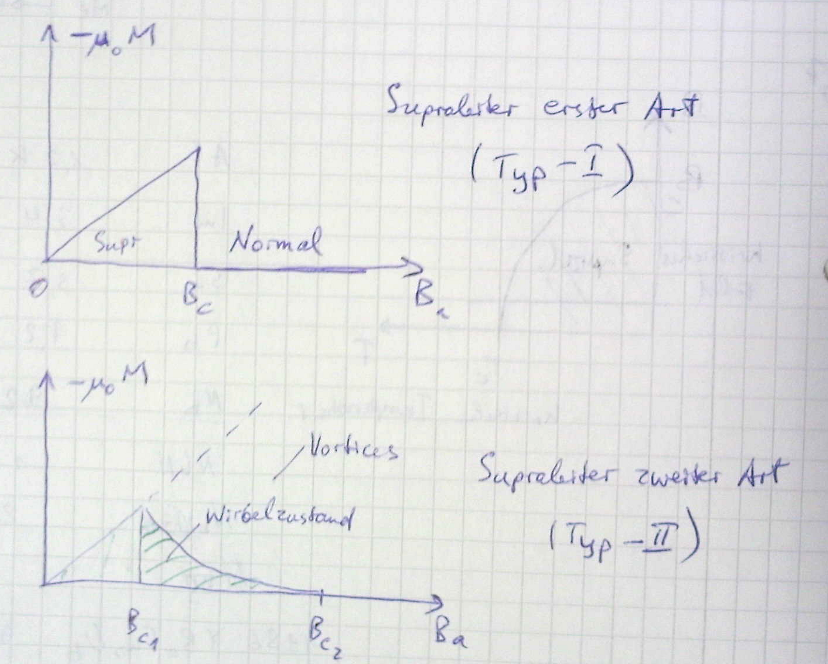
\includegraphics[width=0.75\textwidth]{kap13_04.png}


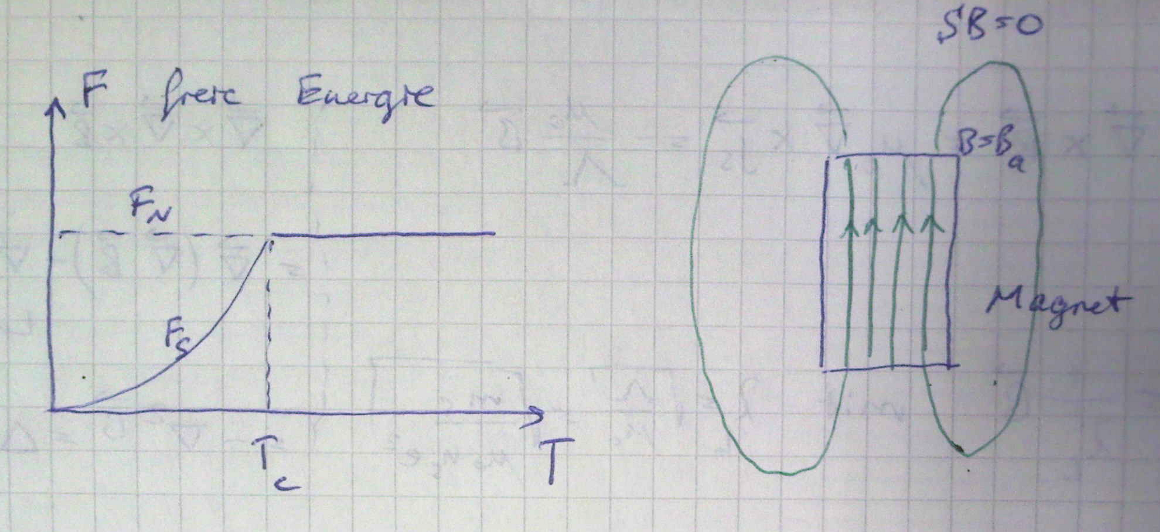
\includegraphics[width=0.75\textwidth]{kap13_05.png}


Arbeit pro Einheitsvolumen der Probe

\[W=-\int_0^{B_a}\vec M\cdot d\vec B_a = \int_0^{B_a} dF_s = \frac{B_a}{\mu_0}dB_a  \]

\[F_S(B_a) - F_S(0) = \frac{B_a^2}{2\mu_0}\]

\section{London-Gleichungen (Postulate)}

\begin{enumerate}
\item[1)] \(\vec E = \frac{\partial}{\partial t}(\Lambda \vec \gamma_S)\) mit \(Lambda = \frac{m_S}{n_Se^2}\)
\item[2)] \(\vec B = -rot(\Lambda \vec j_S)\)
\end{enumerate}

\subsection{Zwei Flüssigkeiten-Modell}

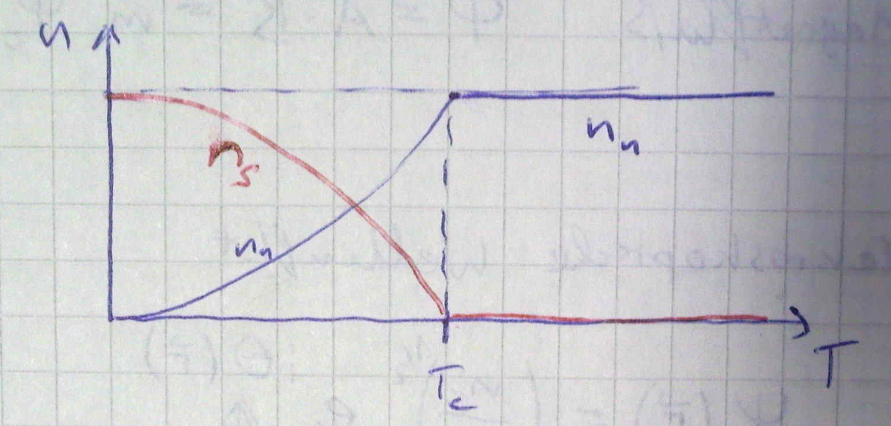
\includegraphics[width=0.75\textwidth]{kap13_06.png}


\[\vec \nabla\times\vec\nabla\times \vec B = \mu_0\vec\nabla\times\vec j_S = -\frac{\mu_0}{\Lambda}\vec B\]

mit \( \vec \nabla\times\vec\nabla\times \vec B = \vec\nabla(\vec \nabla\vec B)-\underbrace{\nabla^2\vec B}_{\text{Laplace}} = -\nabla^2\vec B = \Delta \vec B \)

\[\nabla^2\vec B = \frac{1}{\lambda^2_L}\vec B\]

mit \(\lambda_L = \sqrt{\frac{\Lambda}{\mu_0}} = \sqrt{\frac{m_S}{\mu_0 n_S e^2}}\) als Londonsche eindringtiefe


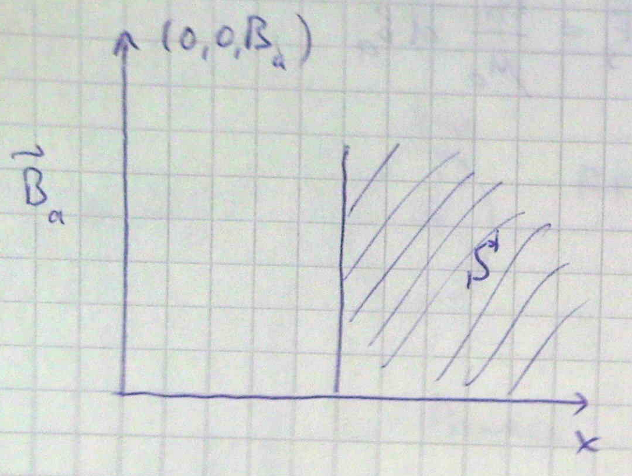
\includegraphics[width=0.75\textwidth]{kap13_07.png}


\[\frac{d^2 B}{dx^2} = \frac{1}{\lambda^2_L}B\]


\[B(x) = B_0e^{-\frac{x}{\lambda_L}}\]


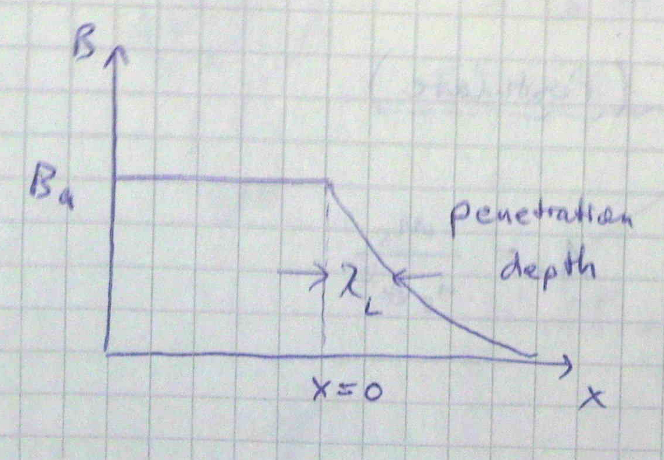
\includegraphics[width=0.75\textwidth]{kap13_08.png}


Für \(B(0) = B_a\), \(B(\infty) = 0\) ergibt sich für \(x>0\):

\[B(x) = B_a e^{-\frac{x}{\lambda_L}}\]


\section{Flußquantisierung}

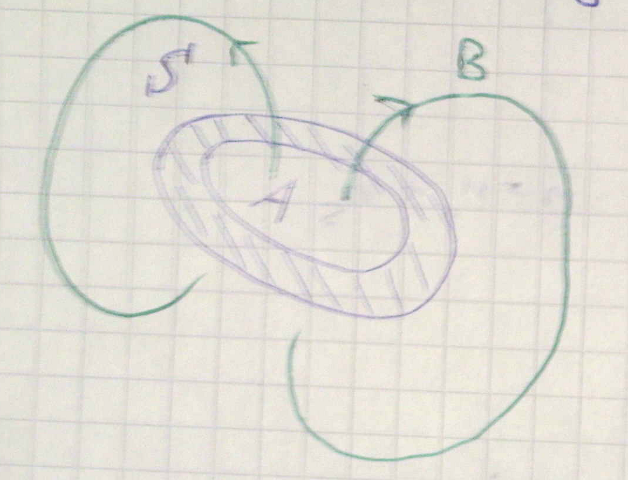
\includegraphics[width=0.45\textwidth]{kap13_09.png}


Magnetfluß \(\Phi = AB = m\Phi_0\), \(\Phi_0 = \frac{h}{2e}=2,7\cdot 10^{-15}V\cdot s\equiv [Wb] \)


Makroskopische Wellenfunktion

\[\Psi(\vec r) \sqrt{\frac{n_S}{2}} e^{i\Theta(\vec r)}\]

Elektronen verhalten sich wie Bosonen-Teilchen


\end{document}
